\chapter{BLE tehnologija}
Bluetooth Low Energy (BLE ili Bluetooth Smart) je be\v{z}i\v{c}ni protokol koji uz pomo\'{c} radiovalova omogu\'{c}uje komunikaciju dva ili vi\v{s}e ure\dj aja. Protokol je prvotno je razvijan od kompanije Nokia pod imenom Wibree, ali 2007. godine dolazi pod jurisdikciju neprofitnog tijela Bluetooth Special Interest Group (SIG) \cite{sig}. SIG je organizacija koja nadgleda razvoj Bluetooth tehnologije i osigurava standardizaciju Bluetooth kompatibilnih ure\dj aja. 2010. godine BLE postaje nova iteracija Bluetooth protokola (verzija 4.0.) iako je u po\v{c}etku bio zami\v{s}ljen kao komplementarni protokol. Aktualna verzija specifikacije je 4.2 \cite{ble_specification}. Na na slici ~\ref{fig:ble} je prikazan logo BLE-a.

\begin{figure}[!htbp]
	\begin{center}
 
\includegraphics[height=3cm,keepaspectratio=true]{ble_logo}
 \caption{Logo BLE protokola}
 \label{fig:ble}
	\end{center}
\end{figure}

Glavna ideja BLE protokola je pru\v{z}iti funkcionanost Bluetooth-a uz \v{s}to manju potro\v{s}nju energije sa ure\dj ajima koji su manji, jeftiniji i optimiziraniji. U mobilnoj industriji Bluetooth protokol je ve\'{c} godinama standard te ga ve\'{c}ina ure\dj aja podr\v{z}ava i korisnici ga koriste koriste u ve\'{c} standradnim primjenama (povezivanje mobitela sa be\v{z}i\v{c}nom slu\v{s}alicom, uparivanje sa automobilom, prijenos podataka izme\dj u ure\dj aja). Me\dj utim, dolaskom BLE-a se podru\v{c}je primjene Bluetooth-a drasti\v{c}no pove\'{c}ava iz razloga \v{s}to je implementacija protokola puno dostupnija zbog slijede\'{c}ih razloga:

\begin{itemize}
	\item Danas gotovo svaki novi pametni telefon na tr\v{z}i\v{s}tu ima BLE \v{c}ip i time je tehnologija dostupa potencijalno ogromnom tr\v{z}i\v{s}tu
	\item \v{C}ipovi su jeftiniji, manji i zahtjevaju manje energije, \v{s}to otvara vrata mnogim novim implementacijama elektroni\v{c}kih ure\dj aja
	\item Protokol je za odre\dj ene primjene br\v{z}i jer za razliku od klasi\v{c}nog Bluetooth-a ne zahtjeva autentikaciju ure\dj aja
\end{itemize}

BLE je temelj za iBeacon tehnologiju, koja pru\v{z}a gotovo identi\v{c}ne funkcionalnosti ali je razvijana od tvrtke Apple pa se shodno tome striktno koristi samo sa Apple-ovim ure\dj ajima.

\section{Arhitektura}

BLE komunikacija se zasniva na radio valovima, u rasponu od 2.4 - 2.2835 GHz, preko kojih se \v{s}alju podatci, podjeljeni na pakete. Frekventni spektar BLE-a je podjeljen na 40 kanala od 2 MHz, te se svaki paket \v{s}alje zasebno kroz kanal \cite{ble_introduction}. Paket se prije slanja modulira GFSK (Gaussian frequency shift modulation) modluacijom i zatim \v{s}alje kroz kanal, teoretski maksimalnom brzinom od 1 Mbit/s (u praksi je to \v{c}esto manje zbog ograni\v{c}enja protokola i komunikacije radio valovima). Potro\v{s}nja energije je dvostruko manja od klasi\v{c}nog Bluetooth-a i iznosi 15 mA pri maksimalnom optere\'{c}enju modula, te se stoga ure\dj aji mogu napajati sa dugmastim baterijama (na ~\ref{fig:ble_baterija} je prikazana baterija koja je napajala BLE ure\dj aj koji je kori\v{s}ten u ovome radu) \v{s}to prili\v{c}no pridonosi prenosivosti, veli\v{c}ini i povoljnosti BLE ure\dj aja.


\begin{figure}[!htbp]
	\begin{center}
 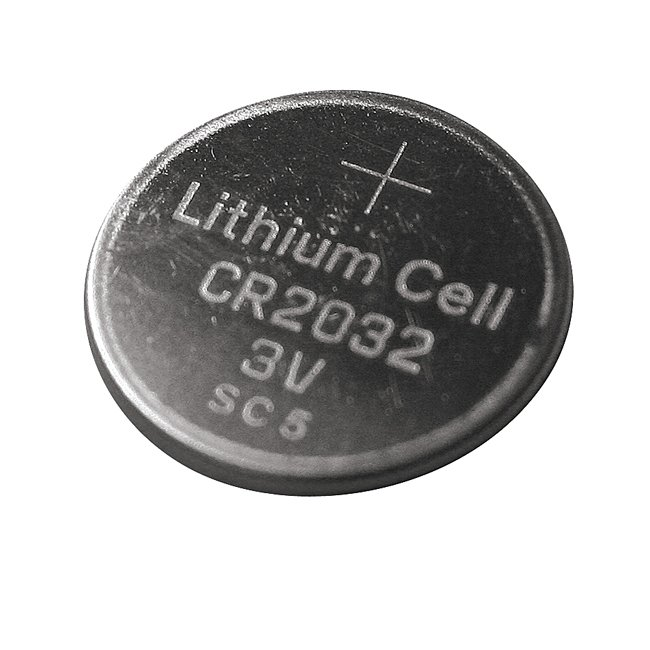
\includegraphics[height=4cm,keepaspectratio=true]{dugmasta_baterija}
 \caption{Dugmasta baterija koja pokre\'{c}e BLE ure\dj aja}
 \label{fig:ble_baterija}
	\end{center}
\end{figure}

Domet protokola u teoriji iznosi \v{c}ak do 100 metara, no u praksi je to do 5 metara iz razloga \v{s}to se cilja na to da ure\dj aji tro\v{s}e \v{s}to manje energije u radu pa se koriste slabije baterije s kojima BLE ure\dj aj ipak ima dovoljno dalek domet za ve\'{c}inu primjena.


\section{Topologija mre\v{z}e}

BLE ure\dj aj mo\v{z}e komunicirati sa drugim ure\dj ajima preko dva na\v{c}ina rada: ogla\v{s}avanje i uparivanje \cite{ble_getting_started}.

\subsection{Ogla\v{s}avanje}

Kod ogla\v{s}avanja ure\dj aj periodi\v{c}ki oda\v{s}ilje signal kojeg detektiraju svi ure\dj ji u dometu. To je jednosmjerna komunikacija i u kojoj razlikujemo oda\v{s}ilja\v{c}a koji konstantno \v{s}alje pakete (uvijek se \v{s}alje standardni paket od 31 B u kojem su osnovne informacije o ure\dj aju, a mogu\'{c}e je slati i dodatni paket sa dodatnim informacijama) i promatra\v{c}a koji konstantno skenira podru\v{c}je koje ga okru\v{z}uje. Ovaj na\v{c}in rada se koristi kada se \v{z}eli s jednim BLE ure\dj ajem slati ista informacija na vi\v{s}e ure\dj aja u dometu. Primjer ovakvog kori\v{s}tenja BLE protokola je proizvod ``Automatic museum guide'' od tvtke Locatify \cite{automatic_museum_guide} . Proizvod uklju\v{c}uje:


\begin{itemize}
	\item Ogla\v{s}iva\v{c}e (BLE ure\dj aje sa baterijom veli\v{c}ine kovanice)
	\begin{itemize}
		\item Postavljaju se u blizini muzejskih eksponata
	\end{itemize}
	\item CMS-a (Content management system)
	\begin{itemize}
		\item Sustav preko kojeg kustosi postavljaju sadr\v{z}aj o eksponatu u audio, video i tekstualnom obliku
	\end{itemize}
	
	\item Personaliziranu mobilnu aplikaciju
	\begin{itemize}
		\item Koriste\'{c}i BLE modul pametnog telefona konstantno skenira prostor i tra\v{z}i ogla\v{s}iva\v{c}e
	\end{itemize}
\end{itemize}

Svrha prozivoda je ta da korisnik sa upaljenom mobilnom aplikacijom dobiva preko pametnog telefona odre\dj eni sadr\v{z}aj kada u\dj e u domet ogla\v{s}iva\'{c}a. To se posti\v{z}e tako da mobilna aplikacija parsira ogla\v{s}iva\v{c}ev paket sa dodatnim podacima i na temelju dobivenih informacija preko CMS-a dobiva odgovaraju\'{c}i sadr\v{z}aj za specifi\v{c}an eksponat.
Prednosti ovakvog ogla\v{s}avanja su brzina i jednostavnost prijenosa, a mana je sigurnost, iz razloga \v{s}to odaslane pakete mogu primiti i ure\dj aji u dometu kojima ti paketi nisu namjenjeni.


\subsection{Uparivanje}
Uparivanje se koristi kod potrebe za sigurnom vezom izme\dj u dva ure\dj aja zbog dvosmjerne komunikacije. Kod komunikacije razlikujemo dvije vrste ure\dj aja:


\begin{itemize}
	\item Centralni ure\dj aj
	\begin{itemize}
		\item Skenira prostor i tra\v{z}i ure\dj aje s kojima mo\v{z}e komunicirati, te kada ih na\dj e inicira komunikaciju
		\item Odre\dj uje pravila komunikacije
	\end{itemize}
	\item Peripetalni ure\dj aj
	\begin{itemize}
		\item Oda\v{s}ilje ogla\v{s}iva\v{c}ke pakete kojima javlja ure\dj ajima u blizini da je spreman za komunikaciju
	\end{itemize}
\end{itemize}

Kada je komunikacija inicirana peripetalni ure\dj aj prestaje oda\v{s}iljati ogla\v{s}iva\v{c}ke pakete i komunicira samo sa centralnim ure\dj ajem. Obi\v{c}ajeni primjer ovakve komunikacije je komunikacija izme\dj u pametnog telefona i ure\dj aja sa nekim senzorom. Jedan od brojnih primjera je proizvod Rhythm+ od tvrtke Scosche \cite{scosche} . Radi se o pametnoj narukvici koja mjeri korisnikov puls te izmjerene podatke \v{s}alje centralnom ure\dj aju (pametnom telefonu sa kompatibilnom aplikacijom koja koristi dobivene podatke za kreiranje svoga sadr\v{z}aja).

Prednost uparivanja, kao na\v{c}ina rada BLE protokola, je sigurnost i optimizacija komunikacije. Ovaj na\v{c}in komunikacije je siguran jer se ure\dj aji moraju prepoznati i upariti da bi uop\'{c}e i moglo do\'{c}i do komunikacije, a optimizacija se posti\v{z}e jer centralni ure\dj aj odre\dj uje pravila komunikacije (koli\v{c}ina podataka koja se \v{s}alje, vremenski intervali u kojima se slanja odvijaju) i samim time se pove\'{c}ava propusnost podataka. Tako\dj er, osigurava se i malena potro\v{s}nja energije jer upareni ure\dj aji \v{s}alju podatke samo kada moraju, za razliku od na\v{c}ina rada gdje se paketi konstantno emitiraju.


\section{Primjena}
Primjena BLE ure\dj aja se temelji na profilu ure\dj aja koji je specificiran od strane SIG-a. Profili su uvedeni s namjerom da BLE ure\dj aji proizvedeni od razli\v{c}itih proizvo\dj a\v{c}a budu standardizirani i me\dj usobno kompatibilni. Tako\dj er, profili garantiraju da ure\dj aj, ovisno o svojoj primjeni, koristi BLE protokol na optimiziran na\v{c}in. Postoje dva op\'{c}a profila koja definiraju osnovna svojstva protokola \cite{ble_getting_started}:

\begin{itemize}
	\item Generic Access Profile (GAP)
	\begin{itemize}
		\item Specificira komunikaciju na najni\v{z}oj razini (ogla\v{s}avanje paketa i skeniranje okoline s ciljem ostvarivanja sigurn konekcije te ostvarivanje i odr\v{z}avanje veze me\dj u ure\dj ajima)
		\item Obavezno ga implementiraju svi BLE ure\dj aji
	\end{itemize}
	\item Generic Attribute Profile (GATT)
	\begin{itemize}
		\item Oslanja se na GAP te na vi\v{s}oj razini definira modele paketa i mehanizme za otkrivanje ure\dj aja i samu komunikaciju
	\end{itemize}
\end{itemize}

Nadalje, SIG je u specifikaciji BLE-a pru\v{z}io i konfiguraciju GATT profila za razna podru\v{c}ja primjene, sve kako bi korisnicima olak\v{s}ali implementaciju protokola u svoje proizvode. Konfiguracija uklju\v{c}uje definiranje komunikacije i na\v{c}ina rada ure\dj aja, kako bi protokol bio \v{s}to optimiziraniji. Neki od najzanimljivijih profila uklju\v{c}uju \cite{ble_profiles}: 


\begin{itemize}
	\item Prona\dj i me profil (FMP)
	\begin{itemize}
		\item Omogu\'{c}uje ure\dj aju da detektira lokaciju drugog ure\dj aja
	\end{itemize}
	
	\item Profil neposredne blizine (PXP)
	\begin{itemize}
		\item Oslanja se na GAP te na vi\v{s}oj razini definira modele paketa i mehanizme za otkrivanje ure\dj aja i samu komunikaciju
	\end{itemize}
	
	\item Profil HID preko GATT-a (HOGP)
	\begin{itemize}
		\item Omogu\'{c}ava slanje HID (Human Interface Device) podataka preko BLE ure\dj aja
		\item Ovaj profil se naj\v{c}e\v{s}\'{c}e koristi za upravljanje tipkovnicama, mi\v{s}evima i daljinskim ure\dj ajima
	\end{itemize}
	
	\item Glukozni profil (GLP)
	\begin{itemize}
		\item Koristi se za mjerenje glukoze kod pacijenata
	\end{itemize}
	
	\item Profil krvnog tlaka (BLP)
	\begin{itemize}
		\item Koristi se za mjerenje krvnog tlaka
	\end{itemize}
	
	\item Profil otkucaja srca (HRP)
	\begin{itemize}
		\item Koristi se za mjerenje otkucaja srca
	\end{itemize}
	
	\item Profil biciklisti\v{c}ke brzine i ritma (CSCP)
	\begin{itemize}
		\item Omogu\'{c}ava pra\'{c}enje brzine i ritma biciklisti\v{c}ke vo\v{z}nje
	\end{itemize}
\end{itemize}

Po navedenim profilima je vidljivo da je primjena BLE-a \v{s}iroka te da se BLE koristi u zdravstvu, sportu i rekreaciji, raznim senzorima i ra\v{c}unalstvu op\'{c}enito.

Za potrebe ovog projekta kori\v{s}ten je Gimbal Proximity Beacon Series 10 BLE ure\dj aj, koji je konfiguriran da radi u PXP profilu. Kupljen je preko internetske trgovine Gimbal \cite{gimbal_beacon} i prikazan na slici ~\ref{fig:gimbal_oglasivac}.

\begin{figure}[!htbp]
	\begin{center}
 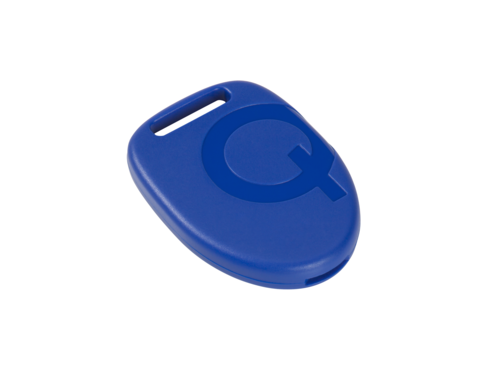
\includegraphics[height=7cm,keepaspectratio=true]{gimbal_s10}
 \caption{Komunikacija dva NFC ure\dj aja}
 \label{fig:gimbal_oglasivac}
	\end{center}
\end{figure}

Specifikacija ogla\v{s}iva\v{c}a:


\begin{itemize}
	\item Dimenzije: 40mm x 28 mm x 5.5 mm
	\item Temperaturni senzor
	\item Udaljenost prijenosa do 50 metara u idealnim uvjetima, u praksi do 10 metara
	\item CR2032 baterija za napajanje
	\item Kompatibilan sa iBeacon tehnologijom

\end{itemize}









